% k4_irrep_decomposition.tex — K4 4-port S-matrix irrep decomposition A1 + T2 (Vol 9 Ch.11)
% Pure TikZ. Matches the CANONICAL leaf k4-port-irrep-decomposition.md:
%   S = (1/2)1 - I, eigenvalues {+1,-1,-1,-1}; A1 (+1) = longitudinal u, c*sqrt2, MASS;
%   T2 (-1,x3) = traceless transverse triplet, speed c.
% 🔴 T2-PHOTON FAMILY CORRECTION 2026-08-02 (Rule 12; the prior header line read
%   "T2 (-1,x3) = microrotational omega, c, PHOTON (and the bound massive mode at saturation)",
%   the prior T2 node read "$\leftrightarrow$ microrotational $\omega$;\;\; speed $c_0$\\
%   \textbf{PHOTON} (free $T_2$); bound massive\\mode at saturation (same $T_2$ sector)", and the
%   prior caption read "the $T_2$ traceless triplet (microrotational $\omega$, $c_0$ --- the
%   photon, whose saturated bound mode is the electron's massive mode)". All three are PRESERVED
%   verbatim here and in git.) Authority: def-t2ph01, ave-kb/common/vocabulary-register.md:851
%   (adjudicated-meaning: "the default canonical 'T2 = the photon' sense is the massless
%   transverse-TRANSLATIONAL mode pair (u-family)"), :858 (sense 1), :859 (sense 2, the gapped
%   Cosserat microrotational omega family -- "This is NOT the photon"), and the watch-list rule at
%   :860 ("never write bare 'T2' or 'T2 microrotational omega' for the photon"). Ruling G2, Grant
%   2026-07-03, research/2026-07-03_g2-photon-relabel_note.md; the KEEP-BOTH adjudication
%   blockquote is at ave-kb/vol1/operators-and-regimes/ch6-universal-operators/
%   k4-port-irrep-decomposition.md:33-35, which states the row's family label is CORRECTED (the
%   massless photon family is transverse-TRANSLATIONAL u, NOT the node micro-rotation) while
%   PRESERVING the :26 row unedited. Decisive receipt: the two massless transverse branches are
%   u-dominated (omega-fraction 2.5e-7, u-fraction 1.000000) and the six gapped branches are
%   omega-dominated (1.000000) -- g2_photon_eigvec_composition.json. The eigenvalues, the
%   A1/T2 split, the speeds (sqrt2*c0 vs c0) and the A1-perp-T2 fence are ALL unchanged; only the
%   DOF-family attribution of the photon is corrected.
\begin{figure}[htbp]
\centering
\begin{tikzpicture}[
    box/.style={draw, rounded corners=3pt, align=center, font=\scriptsize, inner sep=4pt},
    arr/.style={->, thick, gray},
    note/.style={font=\scriptsize, align=left}
]
    % source space
    \node[box, fill=gray!10, minimum width=4.0cm] (src) at (0,2.6)
        {K4 4-port amplitude space\\$S = \tfrac{1}{2}\mathbf{1} - I$ under $T_d$\\eigenvalues $\{+1,\,-1,\,-1,\,-1\}$};

    % A1 branch
    \node[box, fill=green!10, minimum width=4.2cm] (a1) at (-3.0,0.2)
        {$A_1$ (1D, eigenvalue $+1$)\\basis $(1,1,1,1)/2$ — scalar / longitudinal\\$\leftrightarrow$ translational $u$;\;\; speed $\sqrt{2}\,c_0$\\\textbf{MASS / dilatation channel}};

    % T2 branch
    \node[box, fill=blue!10, minimum width=4.4cm] (t2) at (3.0,0.2)
        {$T_2$ (3D, eigenvalue $-1$, triple)\\traceless triplet — vector / transverse\\\textbf{PHOTON} $=$ massless transverse-\\\emph{translational} $u$-family; speed $c_0$\\(\emph{not} the microrotational $\omega$ — that\\family is gapped; \texttt{def-t2ph01})};

    \draw[arr] (src.south) -- (a1.north);
    \draw[arr] (src.south) -- (t2.north);

    % charge/spin note under T2
    \node[note, text width=4.6cm] at (3.0,-1.9)
        {Charge / spin live in the Cosserat $(2,3)$ micro-rotation winding — the \emph{gapped} microrotational $\omega$ family, sense~(2) of the $T_2$ label (CHARGE-``3''); $A_1 \perp T_2$ (\kbleaf{master-equation.md}:20).};

    % Gauss-law asymmetry note under A1
    % 🔴 RULING-21 CORRECTION 2026-08-02 (Rule 12; the prior wording is PRESERVED verbatim here and
    %   in git: "Op3 dissipation: $A_1$ loses energy (Gauss's law forbids longitudinal EM in
    %   vacuum); $T_2$ settles into the quasi-stable photon pattern."). RULING 21 (Grant in-chat
    %   2026-07-19; docket _orchestration/2026-07-10_rulings-docket.md:1809) re-reads Op3's A1
    %   behaviour as LOSSLESS TRANSDUCTION, NOT system dissipation: the A1 MODE empties by a
    %   power-conserving unitary scatter (common-mode rejection redistributes A1 content into the
    %   T2 irreps), and MODE-PROJECTION LOSS != SYSTEM LOSS -- the system conserves power
    %   (src/ave/core/k4_tlm.py:396-398, "Conserves total power"; a lossless reactive scatter with
    %   |Gamma|^2+|T|^2=1 cannot dissipate). Owning KB leaf:
    %   manuscript/ave-kb/vol1/operators-and-regimes/ch6-universal-operators/k4-port-irrep-decomposition.md:28
    %   (corrected Key-Results row, superseded prose preserved inline), :109 (the RULED block),
    %   :199 (blanket reading-note covering the remaining "dissipation" operator labels).
    %   Corroborated at manuscript/ave-kb/common/substrate-native-terminology.md:33 (the licensed
    %   loss/irreversibility channels reduce from FOUR to THREE -- radiative port, boundary-Joule
    %   extraction, Regime-IV rupture -- and Op3 mode-decay is NOT among them) and
    %   manuscript/ave-kb/common/retention-transition-split.md:47 (the canonical MODE-loss worked
    %   example, requires_R = no). The PHYSICS is unchanged -- Gauss's law still forbids
    %   longitudinal EM in vacuum, the A1 mode still empties, only the transverse sector survives.
    %   Only the loss-vs-transduction LABEL is corrected; no number, eigenvalue or speed changes.
    \node[note, text width=4.4cm] at (-3.0,-1.6)
        {Op3 asymmetric \emph{transduction} (RULED 2026-07-19): the $A_1$ \emph{mode} empties into the $T_2$ irreps by lossless power-conserving scatter (Gauss's law forbids longitudinal EM in vacuum) --- mode-projection loss $\neq$ system loss; $T_2$ settles into the quasi-stable photon pattern.};
\end{tikzpicture}
\caption{K4 4-port irrep decomposition $V_{\text{4-port}} = A_1 \oplus T_2$ (Vol.~9 Ch.~11; canonical at \kbleaf{k4-port-irrep-decomposition.md}, \texttt{clm-j550uh}/\texttt{clm-9kd2t3}). The K4-TLM scattering matrix $S = \tfrac{1}{2}\mathbf{1} - I$ splits into the $A_1$ scalar common-mode (longitudinal $u$, $\sqrt{2}\,c_0$ — the mass / dilatation channel) and the $T_2$ traceless triplet ($c_0$). The label $T_2$ names \emph{two} distinct objects (\texttt{def-t2ph01}; Grant ruling G2, 2026-07-03): the \textbf{photon} is sense~(1), the \emph{massless transverse-translational $u$-family}; the \emph{gapped} Cosserat microrotational $\omega$ family is sense~(2) --- the home of the static $(2,3)$ winding and of the electron's bound massive mode at saturation --- and is \emph{not} the photon. The two senses are separated by the massless-vs-gapped mass status. This is the load-bearing $A_1$(mass)/$T_2$(photon) split the mechanical / topological story rests on.}
\label{fig:vol9_k4_irrep_decomposition}
\end{figure}
